\documentclass[11 pt]{article}

\setlength{\oddsidemargin}{-.45in}
%\setlength{\evensidemargin}{-.5in}
\setlength{\textwidth}{7.25in}
\setlength{\topmargin}{-0.95in}
\setlength{\textheight}{10.2in}

\usepackage{graphics}
\usepackage{latexsym}
\usepackage{amsfonts}
\usepackage{amsmath}
\usepackage{amsthm}
\usepackage{epstopdf}
%\usepackage{multicol}
%\usepackage{wrapfig}
\pagestyle{empty}

\usepackage[T1]{fontenc}
\usepackage{baskervald}
\usepackage[bigdelims,vvarbb]{newtxmath} 

\newcommand{\ds}{\ensuremath{\displaystyle}}
\newcommand{\tr}{\vspace{0.5in}}
\newcommand{\lr}{\vspace{1.0in}}
\newcommand{\mr}{\vspace{2.0in}}
\newcommand{\br}{\vspace{3.0in}}

\newcommand{\ps}{Problem Set~}
\newcommand{\vi}{\ensuremath{\mathbf{i}}}
\newcommand{\vj}{\ensuremath{\mathbf{j}}}
\newcommand{\vk}{\ensuremath{\mathbf{k}}}
\newcommand{\vr}{\ensuremath{\mathbf{r}}}
\newcommand{\vecv}{\ensuremath{\mathbf{v}}}
\newcommand{\vu}{\ensuremath{\mathbf{u}}}
\newcommand{\va}{\ensuremath{\mathbf{a}}}
\newcommand{\vs}{\ensuremath{\mathbf{s}}}
\newcommand{\ve}{\ensuremath{\mathbf{e}}}
\newcommand{\vx}{\ensuremath{\mathbf{x}}}
\newcommand{\vc}{\ensuremath{\mathbf{c}}}
\newcommand{\vb}{\ensuremath{\mathbf{b}}}

\usepackage{hyperref} 
\hypersetup{colorlinks=true, linkcolor=blue,  anchorcolor=blue,  
citecolor=blue, filecolor=blue, menucolor=blue, pagecolor=blue,  
urlcolor=blue,pdftitle={MTH 202 Checkpoint}}

\usepackage{framed}

\newcommand{\bdr}{\ensuremath{\mathbb{R}}}

\newcommand{\be}{\begin{enumerate}}
\newcommand{\ee}{\end{enumerate}}

\newcommand{\bi}{\begin{itemize}}  
\newcommand{\ei}{\end{itemize}}

%\renewcommand{\baselinestretch}{1.5}


\begin{document}
 \hfill Boelkins \\
 
\begin{center}
Math 202-06 \\
{\bf Checkpoint 9}
\end{center}


\noindent {\bf Directions:}

\begin{itemize}
	
	\item {\bf Desmos.} You may use \href{https://www.desmos.com/calculator}{\emph{Desmos}} for computations and graphing, just like we do during class.  Any work done in \emph{Desmos} must be summarized and briefly explained in writing on your paper.  
	
	\item {\bf Resources.} During each checkpoint, you may access your own 1 page of study notes, plus \emph{Desmos}; no other uses of your computer or tablet are permitted unless specified directly.  No collaboration with other human beings or other internet resources are allowed.
	
%	\emph{Note well: if you collaborate with someone else, it is often obvious that collaboration has occurred.  Please do not put your academic standing at risk by doing this.}
	
	\item {\bf Competence.} Each week, your goal is to demonstrate competence on as many of the included learning targets as you can.  Each question will be marked either ``Y'' or ``NY'': Y for ``yes'', NY for ``not yet''.  Every learning target will appear on three different checkpoints, so you'll have multiple attempts to demonstrate your understanding.  ``Competence'' is defined as work that demonstrates clear and complete understanding of the relevant concepts in the learning target. While the work may include a minor error, or one or two minor steps may not be well explained, otherwise the work is complete, correct, and convincing, including the proper use of notation, and appropriate explanation of meaning that uses correct terminology.  (On rare occasions, you might get a ``NY*''; such a mark means you are close to competence and that you have the option to have a short conversation with me prior to the next Checkpoint and attempt to demonstrate ``Y''-level understanding through the conversation aloud.)	
\end{itemize}

\noindent \hrulefill \\

\noindent {\bf Learning Targets:} For Checkpoint \#9, there are four learning targets being assessed: 

\begin{quote}
{\bf LT 8}: I can use definite integrals to represent key quantities in applications such as the work done by a varying force or the pressure that water exerts against a dam. (Section 6.4)
\end{quote}

\begin{quote}
{\bf LT 9}: I can check whether a function is a solution to a differential equation and explain why the function is or is not a solution.  (Section 7.1)
\end{quote}

\begin{quote}
{\bf LT 10}:  I can apply Euler’s Method to generate an approximate solution to an initial value problem and explain the result’s meaning in context.
\end{quote}

\begin{quote}
{\bf LT 11}:  I can express real world situations as differential equations, determine any stable or unstable equilibrium solutions, and explain the significance of the equilibrium solutions in context.
\end{quote}

\noindent \hrulefill \\

\vfill \hfill {\bf OVER} 

\pagebreak

\noindent Name: \\ 

\noindent To demonstrate competence on Learning Target \#$n$, you need to correctly respond to all or nearly all of the prompts in question \#$n$.  

\begin{enumerate}

% {\bf LT 8}: I can use definite integrals to represent key quantities in applications such as the work done by a varying force or the pressure that water exerts against a dam. (Section 6.4)

\item[8.] Consider a trough with a triangular end as pictured below.  


%Assume the trough is 16 feet wide along its top, 20 feet deep, 30 feet long, and that it is full of water to a depth of 17 feet.   As usual, the weight density of water is 62.4 pounds per cubic foot.

Assume the trough is 12 feet wide along its top, 15 feet deep, 18 feet long, and that it is full of water to a depth of 13 feet.   As usual, the weight density of water is 62.4 pounds per cubic foot.

\be

	\item \emph{Determine the total amount of hydrostatic force on one end of the trough}.  Clearly show relevant slices that go in to determining the definite integral that answers the question. State the appropriate definite integral clearly and evaluate it using technology to determine the total work to achieve the task noted above.  Include units on your result.

\hfill \scalebox{0.4}{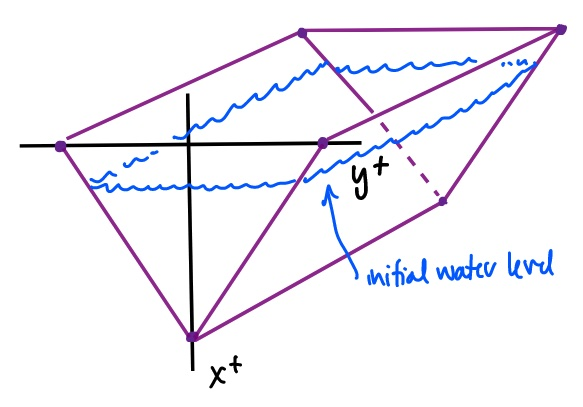
\includegraphics{images/LT-8-tank-3}}

\tr

%v1 - Determine the total amount of work that would be required to empty the tank until 4 feet of water remains in it, while pumping the water to a truck whose tank is 2 feet above the top of the tank}

%v2 - Determine the total amount of work that would be required to empty the tank until 3 feet of water remains in it, while pumping the water to a truck whose tank is 6 feet above the top of the tank}

	\item \emph{Determine the total amount of work that would be required to empty the tank until 3 feet of water remains in it, while pumping the water to a truck whose tank is 6 feet above the top of the tank}.  In your response, clearly show the relevant slice(s) and computations that are involved in determining the definite integral that answers the question.  State the appropriate definite integral clearly and evaluate it using technology to determine the total work to achieve the task noted above.  Include units on your result.
	
\hfill \scalebox{0.4}{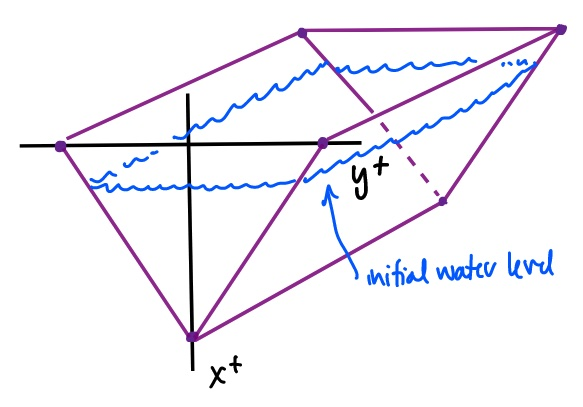
\includegraphics{images/LT-8-tank-3}}

\lr
	

\ee  


\pagebreak

\noindent Name: \\ 

%{\bf LT 10}: I can check whether a function is a solution to a differential equation and explain why the function is or is not a solution.

\item[9.] For each of the following prompts, determine whether or not the given function is or is not a solution to the given differential equation.  For each, show your computational/algebraic work and write a brief sentence to clearly justify your conclusion.
	
	
	\be
		\item $\frac{dM}{dt} = 0.1M - 10$, $M(t) = 100 + 5e^{0.1t}$
		%$y(t) = \frac{1}{3}t^3 + e^{2t} + 5$; $\frac{dy}{dt} = t^2 + e^{2t}$		
	
		\lr \tr \tr
	
		\item $\frac{dQ}{dt} = -4Q$, $Q(t) = \sin(4t)$
		%$P(t) = 4$; $\frac{dP}{dt} = -3P(4-P)$
		
		\lr \tr \tr
		
		\item $\frac{dy}{dt} = -4t$, $y(t) = -2t^2 + 4t + 4$
		%$F(t) = 70 + 25e^{-0.1t}$; $\frac{dF}{dt} = -\frac{1}{10}F  + 7$
		
		\lr \tr \tr
		
		\item $\frac{dP}{dt} = -0.05 P (20 - P)$, $P(t) = 20$
		%$A(t) = \cos(2t)$; $\frac{dA}{dt} = -2A$
		
		\lr \tr
		

	\ee
	
	\ \vfill

\pagebreak

\pagebreak

% {\bf LT 11}:  I can apply Euler’s Method to generate an approximate solution to an initial value problem and explain the result’s meaning in context.

\item[10.] Consider the initial value problem $\frac{dy}{dx} = -0.6x + 0.4y$, $y(0) = 1$.

Apply Euler's Method with $\Delta x = 0.25$ to estimate $y(0.75)$.  

Clearly show your work and thinking below (that is, show how at least one row in your table is determined), and fill in the given table accordingly (there are more rows in the table than you'll need; you decide how many rows you need).  Write at least one sentence to summarize your work and your final answer to the main question posed.


\lr \lr

\begin{center}
\begin{tabular}{|c|c|c|c|c|}
\hline
$\Delta x$ & $x$ & $y$ &  Slope   &  $\Delta y$ \\
\hline
  \ \hspace{0.5in} \ & \ \hspace{0.5in} \  & \ \hspace{0.5in} \  & \  \hspace{0.5in} \ & \  \hspace{0.5in} \ \\   \hline  
  \ & \ & \ & \ & \ \\ \hline
    \ & \ & \ & \ & \ \\  \hline
  \ & \ & \ & \ & \ \\  \hline
   \ & \ & \ & \ & \ \\   \hline
   \ & \ & \ & \ & \ \\   \hline   
   \ & \ & \ & \ & \ \\  
\hline
\end{tabular}
\end{center}

\pagebreak

%{\bf LT 12}:  I can express real world situations as differential equations, determine any stable or unstable equilibrium solutions, and explain the significance of the equilibrium solutions in context. (Section 7.5)

% do a mixing problem

\item[11.]  

\be
	\item Suppose that saltwater is entering and exiting a 500L tank in the following way:  solution concentrated at 6 g/L enters the tank at a rate of 4 L/min, and perfectly mixed solution exits the tank at a rate of 4 L/min.  Let $S(t)$ represent the number of grams of salt in the tank at time $t$.
	
	\be
		\item Set up a differential equation whose solution is $S(t)$.  Write to demonstrate your thinking.
		\lr \tr
		
		\item What is the equilibrium solution to the differential equation you determined?  Why does this make sense?  Explain.
		\lr \tr
		
	\ee
	
	
	\item A pie removed from an oven cools at a rate proportional to the difference between the pie's temperature and the temperature of the surrounding room, which is 70 degrees F.  Let $P(t)$ be the pie's Fahrenheit temperature, and say that the proportionality constant is $k = 0.05$.  
	
	\be
		\item Set up a differential equation whose solution is $P(t)$.  Write to demonstrate your thinking; in particular, be sure to address the role of any minus signs in the differential equation.
		\lr \tr
		
		\item What is the equilibrium solution to the differential equation you determined?  Why does this make sense?  Explain.
		\lr
	\ee
	
	\item Choose one of the two equilibrium solutions you found above.  Is the solution stable or unstable?  Why?
	
\ee

	
\end{enumerate}
\end{document}